\documentclass[11pt,a4paper]{article}
\usepackage[utf8]{inputenc}
\usepackage[T1]{fontenc}
\usepackage{lmodern}
\usepackage{amsmath,amssymb,amsfonts,bm}
\usepackage{graphicx}
\usepackage{booktabs}
\usepackage{microtype}
\usepackage{geometry}
\geometry{a4paper, margin=2.5cm, top=2.8cm, bottom=2.8cm}
\usepackage[numbers,sort&compress]{natbib}
\usepackage{hyperref}
\hypersetup{
    colorlinks=true,
    linkcolor=blue,
    citecolor=blue,
    urlcolor=blue
}

\title{\textbf{Microstates and Macroscopic Thermodynamics of a Binary System}\\[0.5em]
\large Statistical Physics --- Laboratory Practice 1}
\author{\textbf{Andr\'es M\'armol del Amo} \and \textbf{H\'ector Armenteros Arauzo} \and \\
\textbf{Carlos Cordero L\'opez} \and \textbf{Guillermo Garc\'ia Pelayo}\\[0.6em]
\small Section 1 -- Group C, Department of Physics, Universidad Carlos III de Madrid}
\date{\today}

\begin{document}
\maketitle

\begin{abstract}
We investigate the microscopic foundations of statistical mechanics and the emergence of macroscopic thermodynamic behavior using an idealized binary system of $N$ unbiased, independent particles (two-state model isomorphic to spin-$1/2$ paramagnetic dipoles and binary lattice gases). The accessible phase space expands exponentially as $2^N$, exhibiting a fundamental tension between microscopic reversibility and macroscopic irreversibility. We implement and evaluate two complementary computational paradigms: (i) full bitwise microstate enumeration with constant-memory bit-shifting and vectorized popcounts, measuring exact state distributions up to a computational frontier of $N_{\max} = 36$ under a strict 5-minute wall-clock constraint; and (ii) log-space combinatorics based on the log-Gamma function ($\ln\Gamma$), overcoming IEEE-754 64-bit floating-point overflow ($N > 1029$) to probe distributions up to macroscopic scales ($N \sim 10^{23}$). For a team-specific system size of $N = 100 + M$, we compute macrostate multiplicities $\Omega(N, k)$, probability profiles, and Boltzmann entropy differences $\Delta S = k_B \ln[\Omega(k_1)/\Omega(k_2)]$. In accordance with the de~Moivre--Laplace limit, relative macroscopic fluctuations decay as $\sigma/N \propto 1/\sqrt{N}$, confining the system to an overwhelmingly probable equilibrium state. Finally, recurrence times for low-entropy configurations demonstrate that spontaneous violations of the Second Law of Thermodynamics are not dynamically prohibited, but statistically impossible on cosmological timescales.
\end{abstract}

\vspace{0.5em}
\noindent\textbf{Keywords:} Statistical mechanics, microstates, macrostate distribution, Boltzmann entropy, de~Moivre--Laplace theorem, thermodynamic limit.

\noindent\textbf{Source Code \& Audit Repository:} \url{https://github.com/guillergape/StatPhys_Lab1_S1_GroupC}

\vspace{1.5em}

% ==============================================================================
% SECTION 1: INTRODUCTION & OBJECTIVES
% ==============================================================================
\section{Introduction \& Objectives}
\label{sec:intro}

Statistical mechanics bridges the deterministic microscopic laws governing individual particles and the phenomenological, macroscopic laws of thermodynamics. While classical thermodynamics operates through bulk state variables such as temperature $T$, pressure $P$, volume $V$, and internal energy $U$, statistical mechanics demonstrates that these quantities represent statistical averages over a colossal number of microscopic configurations.

\subsection{Theoretical Foundations}
Consider an isolated system composed of $N$ distinguishable, non-interacting binary units, where each unit can occupy one of two discrete states, conventionally labeled as heads ($\sigma_i = 1$) or tails ($\sigma_i = 0$). This simple model serves as the archetypal paradigm for diverse physical systems, including:
\begin{itemize}
    \item Non-interacting spin-$1/2$ paramagnets in an external magnetic field $B$, where magnetic moments point parallel ($\mu$) or antiparallel ($-\mu$) to the field;
    \item Lattice gases with site occupancy numbers $n_i \in \{0, 1\}$;
    \item Two-level quantum systems in thermal equilibrium.
\end{itemize}

A \textbf{microstate} $\bm{\sigma} = (\sigma_1, \sigma_2, \dots, \sigma_N) \in \{0, 1\}^N$ specifies the precise microscopic configuration of every individual degree of freedom. For $N$ independent entities, the total number of accessible microstates in phase space is:
\begin{equation}
    \Omega_{\text{total}} = 2^N.
    \label{eq:total_microstates}
\end{equation}
Under the \textit{Fundamental Postulate of Statistical Mechanics}, an isolated system in thermodynamic equilibrium is equally likely to be found in any of its accessible microstates. Thus, for an unbiased coin system, each individual microstate carries an identical a priori probability:
\begin{equation}
    P(\bm{\sigma}) = \frac{1}{\Omega_{\text{total}}} = \frac{1}{2^N}.
\end{equation}

Conversely, a \textbf{macrostate} is characterized exclusively by coarse-grained, macroscopic observables. For our system, the natural macrostate descriptor is the total number of heads $k$:
\begin{equation}
    k = \sum_{i=1}^{N} \sigma_i, \qquad k \in \{0, 1, \dots, N\}.
\end{equation}
The number of distinct microstates corresponding to a given macrostate $k$ defines its \textbf{multiplicity} (or thermodynamic weight) $\Omega(N, k)$, given by the binomial coefficient:
\begin{equation}
    \Omega(N, k) = \binom{N}{k} = \frac{N!}{k!\,(N - k)!}.
    \label{eq:binomial_multiplicity}
\end{equation}
Consequently, the probability of observing the macrostate $k$ upon random sampling is:
\begin{equation}
    P(N, k) = \frac{\Omega(N, k)}{2^N} = \binom{N}{k} 2^{-N}.
    \label{eq:macrostate_probability}
\end{equation}

The connection to macroscopic thermodynamics is established via Ludwig Boltzmann's entropy postulate:
\begin{equation}
    S(N, k) = k_B \ln \Omega(N, k),
    \label{eq:boltzmann_entropy}
\end{equation}
where $k_B = 1.380649 \times 10^{-23}\,\text{J}\cdot\text{K}^{-1}$ is the Boltzmann constant. In statistical mechanics, entropy is directly proportional to the logarithmic volume of accessible phase space associated with a macrostate. The principle of maximum entropy (and hence the Second Law of Thermodynamics) states that an unconstrained system evolves toward the macrostate with the highest multiplicity, which corresponds to the state of maximum molecular disorder.

In the \textbf{thermodynamic limit} ($N \to \infty$ or $N \sim 10^{23}$ particles), the central limit theorem (specifically the de~Moivre--Laplace theorem) dictates that the discrete binomial distribution converges asymptotically to a continuous Gaussian:
\begin{equation}
    \Omega(N, k) \simeq 2^N \sqrt{\frac{2}{\pi N}} \exp\left[ -\frac{2\,(k - N/2)^2}{N} \right],
    \label{eq:gaussian_limit}
\end{equation}
with mean $\mu = N/2$ and standard deviation $\sigma = \sqrt{N}/2$. Although the absolute spread $\sigma \propto \sqrt{N}$ increases with system size, the relative fluctuation scale:
\begin{equation}
    \frac{\sigma}{N} = \frac{1}{2\sqrt{N}} \xrightarrow[N \to \infty]{} 0
\end{equation}
diminishes to zero. For macroscopic systems ($N \sim 10^{23}$), relative fluctuations are suppressed to $\sim 10^{-12}$, transforming statistical probabilities into deterministic physical certainties.

\subsection{Laboratory Objectives}
The primary objective of this experimental and computational investigation is to explore the transition from discrete microscopic counting to macroscopic thermodynamic laws. Specifically, we set out to:
\begin{enumerate}
    \item \textbf{Exact Bitwise Microstate Enumeration:} Implement a constant-memory generator utilizing bitwise arithmetic and popcount operations to enumerate all $2^N$ microstates for small systems ($N = 7$), verify multiplicities against Pascal's triangle, and experimentally determine the maximum system size $N_{\max}$ achievable within a 5-minute wall-clock threshold.
    \item \textbf{Log-Space Combinatorics and Overflow Bypass:} Formulate a numerically stable evaluation of $\ln\Omega(N, k)$ using the log-Gamma function ($\ln\Gamma$) to compute macrostate distributions for large $N$ ($N = 20, 50, 80, 100$) where standard 64-bit floating-point variables experience catastrophic numerical overflow ($N > 1029$).
    \item \textbf{Probabilities and Macrostate Thermodynamics:} For a group-specific system size $N = 100 + M$ (where $M$ is derived from the harmonic mean of the team members' university IDs), calculate exact macrostate probabilities, central symmetric confidence intervals, and evaluate Boltzmann entropy differences $\Delta S = k_B \Delta(\ln\Omega)$.
    \item \textbf{Statistical Irreversibility and the Second Law:} Quantify the expected recurrence time required to spontaneously produce an ordered low-entropy state ($k = 8$) under continuous physical coin-tossing, comparing the result with the cosmological age of the Universe ($\tau_U \approx 13.8 \times 10^9\,\text{yr}$).
    \item \textbf{Thermodynamic Limit Asymptotics:} Apply Stirling's approximation to analytically evaluate the system's behavior as $N \to 10^{23}$, demonstrating the mathematical necessity of the Second Law of Thermodynamics in macroscopic physics.
\end{enumerate}

% ==============================================================================
% SECTION 2: METHODOLOGY & COLLABORATIVE WORKFLOW
% ==============================================================================
\section{Methodology \& Collaborative Workflow}
\label{sec:methodology}

Scientific computing requires strict adherence to reproducible environments, modular software engineering, version-controlled collaboration, and exhaustive verification. Our methodology integrates modern industry standards with academic rigor.

\subsection{Reproducible Computational Environment}
To eliminate platform discrepancies across team workstations (running macOS, Linux, and Windows), all computational analyses are executed within an isolated, deterministic Conda environment named \texttt{statphys\_lab1}. The complete environment specification is codified in \texttt{environment.yml}:
\begin{itemize}
    \item \textbf{Python 3.11.9}: Serves as the base runtime, providing native support for \texttt{int.bit\_count()} and optimized integer arithmetic.
    \item \textbf{NumPy ($\ge 1.24$)}: Utilized for high-performance vectorized operations, contiguous memory arrays (\texttt{numpy.arange}), and C-accelerated bitwise counting (\texttt{numpy.bitwise\_count}).
    \item \textbf{SciPy ($\ge 1.10$)}: Provides the specialized logarithmic gamma function \texttt{scipy.special.gammaln} for array-wide log-space combinatorics.
    \item \textbf{Matplotlib ($\ge 3.7$)}: Configured for the publication-quality generation of vector graphic figures (\texttt{.pdf}) with explicit typographical scaling.
    \item \textbf{Pytest ($\ge 7.0$)}: Automated unit testing framework executed across all modules prior to code integration.
\end{itemize}

\subsection{Modular Architecture \& Shared Interfaces}
The codebase is decoupled into distinct modules under \texttt{src/}, each adhering to strict, pre-agreed type-annotated signatures defined in \texttt{PLAN.md}:
\begin{itemize}
    \item \texttt{src/microstates.py}: Defines \texttt{microstates(N: int) -> Iterator[int]} and \texttt{macrostate\_counts(N: int) -> list[int]}. Implements both pure-Python bitwise generation and multi-threaded block-vectorized chunking for execution benchmarks.
    \item \texttt{src/combinatorics.py}: Defines \texttt{ln\_omega(N: int, k: int) -> float} based on \texttt{math.lgamma}, vectorized array utilities, and asymptotic Gaussian approximations.
    \item \texttt{src/thermodynamics.py}: Defines functions for calculating the team parameter $N = 100 + M$, macrostate probabilities \texttt{probability(N, k)}, cumulative interval probabilities \texttt{interval\_probability(N, k1, k2)}, and entropy differences \texttt{delta\_entropy(N, k1, k2)}.
    \item \texttt{main.py}: Master pipeline executing all computational routines sequentially, printing validated numerical tables and rendering vector plots directly to \texttt{report/figures/}.
\end{itemize}

\subsection{Version Control, Feature Branching, and Peer Review}
Collaboration is governed by a distributed Git workflow hosted on GitHub. Direct commits to the \texttt{main} branch are strictly restricted. Instead, a structured feature-branch workflow is enforced:
\begin{enumerate}
    \item Work is divided into discrete, ordered phases allocated among team members.
    \item Each member works in an isolated branch (e.g., \texttt{feature/bitwise-enumeration}, \texttt{feature/log-combinatorics}, \texttt{feature/latex-report}).
    \item Cross-review protocol: Once a phase is complete, a formal Pull Request (PR) is opened against \texttt{main}. A designated teammate reviews the implementation against analytical benchmarks and verifies that all unit tests pass before approval and merge.
\end{enumerate}

\subsection{Verification and Unit Testing Suite}
Reproducibility is enforced via automated test suites located in \texttt{tests/}. Every algorithm is validated against theoretical invariants:
\begin{itemize}
    \item \textbf{Conservation of States:} Verification that $\sum_{k=0}^{N} \Omega(N, k) \equiv 2^N$.
    \item \textbf{Reflection Symmetry:} Invariance under heads-tails exchange, $\Omega(N, k) \equiv \Omega(N, N - k)$.
    \item \textbf{Exact Comparison:} Comparison of $\exp[\ln\Omega(N, k)]$ against exact arbitrary-precision integer combinatorics (\texttt{math.comb(N, k)}) for all $k \le N \le 100$, confirming a relative error $|e^{\ln\Omega} - \binom{N}{k}|/\binom{N}{k} < 10^{-11}$.
    \item \textbf{Boundary Limits:} Exact validation at extremities: $\Omega(N, 0) = \Omega(N, N) = 1$ and $\Omega(N, 1) = N$.
\end{itemize}

\subsection{AI Assistance Governance \& Audit Trail}
In full compliance with Universidad Carlos III de Madrid academic regulations and Phase 3 of the Laboratory Project Guidelines, artificial intelligence systems (Claude Code, GitHub Copilot, and Google Antigravity) are utilized strictly as collaborative development tools. To maintain complete academic integrity, every interaction is audited in \texttt{AI\_STATEMENT.md}, recording:
\begin{enumerate}
    \item The verbatim prompt submitted by the team member;
    \item The code, LaTeX, or documentation synthesized by the assistant;
    \item The rigorous verification procedures, modifications, and unit tests independently executed by the authors.
\end{enumerate}

% ==============================================================================
% SECTION 3: COMPUTATIONAL ANALYSIS OF MICROSTATES
% ==============================================================================
\section{Computational Analysis of Microstates}
\label{sec:microstates}

% Phase 2 (Guillermo): Part 1 a, b. Every number here comes from src/microstates.py.
\subsection{Enumeration of microstates}
Each microstate of $N$ coins is stored as an integer $s\in\{0,\dots,2^N-1\}$ whose bit $i$ is coin $i$ (1 = heads, 0 = tails). The generator \texttt{microstates(N)} runs over \texttt{range(1 << N)} and yields one state at a time, so memory does not grow with $N$; the macrostate of a state is its number of set bits, $k=$ \texttt{s.bit\_count()}. Counting the states per $k$ gives $\Omega(N,k)$, checked against $\binom{N}{k}$ for $N\le 15$ and against Table~1 of the manual for $N=5$.

\paragraph{(a) $N=7$.} Table~\ref{tab:n7} lists the $2^7=128$ microstates grouped by macrostate. The multiplicities are exact integers (no uncertainty) and follow row 7 of Pascal's triangle: symmetric under heads $\leftrightarrow$ tails and largest at $k=3,4$.

\begin{table}[htbp]\centering\small
\caption{All microstates of $N=7$ coins grouped by macrostate (H = heads, T = tails, coin 0 first).}\label{tab:n7}
\begin{tabular}{@{}p{0.17\textwidth}p{0.68\textwidth}r@{}}
\toprule
Macrostate & Microstates & $\Omega(7,k)$ \\
\midrule
7 heads, 0 tails & \texttt{HHHHHHH} & 1 \\
6 heads, 1 tail & \texttt{HHHHHHT, HHHHHTH, HHHHTHH, HHHTHHH, HHTHHHH, HTHHHHH, THHHHHH} & 7 \\
5 heads, 2 tails & \texttt{HHHHHTT, HHHHTHT, HHHTHHT, HHTHHHT, HTHHHHT, THHHHHT, HHHHTTH, HHHTHTH, HHTHHTH, HTHHHTH, THHHHTH, HHHTTHH, HHTHTHH, HTHHTHH, THHHTHH, HHTTHHH, HTHTHHH, THHTHHH, HTTHHHH, THTHHHH, TTHHHHH} & 21 \\
4 heads, 3 tails & \texttt{HHHHTTT, HHHTHTT, HHTHHTT, HTHHHTT, THHHHTT, HHHTTHT, HHTHTHT, HTHHTHT, THHHTHT, HHTTHHT, HTHTHHT, THHTHHT, HTTHHHT, THTHHHT, TTHHHHT, HHHTTTH, HHTHTTH, HTHHTTH, THHHTTH, HHTTHTH, HTHTHTH, THHTHTH, HTTHHTH, THTHHTH, TTHHHTH, HHTTTHH, HTHTTHH, THHTTHH, HTTHTHH, THTHTHH, TTHHTHH, HTTTHHH, THTTHHH, TTHTHHH, TTTHHHH} & 35 \\
3 heads, 4 tails & \texttt{HHHTTTT, HHTHTTT, HTHHTTT, THHHTTT, HHTTHTT, HTHTHTT, THHTHTT, HTTHHTT, THTHHTT, TTHHHTT, HHTTTHT, HTHTTHT, THHTTHT, HTTHTHT, THTHTHT, TTHHTHT, HTTTHHT, THTTHHT, TTHTHHT, TTTHHHT, HHTTTTH, HTHTTTH, THHTTTH, HTTHTTH, THTHTTH, TTHHTTH, HTTTHTH, THTTHTH, TTHTHTH, TTTHHTH, HTTTTHH, THTTTHH, TTHTTHH, TTTHTHH, TTTTHHH} & 35 \\
2 heads, 5 tails & \texttt{HHTTTTT, HTHTTTT, THHTTTT, HTTHTTT, THTHTTT, TTHHTTT, HTTTHTT, THTTHTT, TTHTHTT, TTTHHTT, HTTTTHT, THTTTHT, TTHTTHT, TTTHTHT, TTTTHHT, HTTTTTH, THTTTTH, TTHTTTH, TTTHTTH, TTTTHTH, TTTTTHH} & 21 \\
1 head, 6 tails & \texttt{HTTTTTT, THTTTTT, TTHTTTT, TTTHTTT, TTTTHTT, TTTTTHT, TTTTTTH} & 7 \\
0 heads, 7 tails & \texttt{TTTTTTT} & 1 \\
\midrule
Total & & 128 \\
\bottomrule
\end{tabular}
\end{table}

\paragraph{(b) Largest $N$ that can be fully enumerated.} We timed the full enumeration and histogram of all $2^N$ states (\texttt{time.perf\_counter}, peak memory with \texttt{tracemalloc}) for growing $N$ on a laptop with an Intel Core i7-1255U (12 threads) and 15.7\,GB of RAM. Two versions were tested, both of which build every microstate and count its heads:
\begin{itemize}
\item the pure-Python generator \texttt{macrostate\_counts}: $750$--$780$\,ns per state, constant memory (no traced allocation);
\item \texttt{macrostate\_counts\_fast}: the same enumeration in blocks of $2^{22}$ consecutive integers (\texttt{numpy.arange}), heads counted with \texttt{numpy.bitwise\_count} and histogrammed with \texttt{numpy.bincount}, the range $0\dots2^N-1$ split among the 12 CPU threads. Memory is fixed by the block size: $71$\,MB per process measured, independent of $N$.
\end{itemize}

\begin{table}[htbp]\centering\small
\caption{Wall-clock time of the full enumeration with \texttt{macrostate\_counts\_fast} (one run per $N$; the time per state varies by about $\pm10\%$ between runs).}\label{tab:benchmark}
\begin{tabular}{@{}rrrr@{}}
\toprule
$N$ & $2^N$ & Time (s) & Time per state (ns) \\
\midrule
30 & $1.07\times10^{9}$ & 3.3 & 3.0 \\
31 & $2.15\times10^{9}$ & 5.5 & 2.6 \\
32 & $4.29\times10^{9}$ & 10.9 & 2.5 \\
33 & $8.59\times10^{9}$ & 23.6 & 2.7 \\
34 & $1.72\times10^{10}$ & 41.4 & 2.4 \\
35 & $3.44\times10^{10}$ & 85.5 & 2.5 \\
36 & $6.87\times10^{10}$ & 156.2 & 2.3 \\
\bottomrule
\end{tabular}
\end{table}

\textbf{Result: $N_{\max}=36$} within 5 minutes ($156$\,s, Table~\ref{tab:benchmark}). Each extra coin doubles the work, so $N=37$ is predicted at $2^{37}\times(2.3\pm0.2)\,\text{ns}\approx310\pm30$\,s, above the limit. With the plain generator the limit is $N=28$ ($2^{28}\times0.76\,\mu\text{s}\approx200$\,s; $N=29$ would take $\approx410$\,s).

\textbf{Limiting factor: time, not memory.} Because the states are generated on the fly and never stored, memory stays constant and the only constraint is the $2^N$ growth of the number of operations: at $2.3$\,ns per state, $N=40$ needs $\approx42$\,min, $N=50$ about a month and $N=100$ about $10^{14}$ years. Memory would become the limit only if the states were kept: a Python list of $2^N$ integers costs $\approx36$\,B per state, which fills the 15.7\,GB of RAM at $N\approx28$, and writing the $2^{36}$ states of $N_{\max}$ as text would take $\approx2.5$\,TB of disk. The fast version gains a factor $\approx330$ over the generator (vectorised popcount in C, $\times100$; 12 threads, $\times3$ since the threads share the memory bandwidth), which is worth only $\log_2 330\approx8$ more coins: exponential growth makes any constant speed-up almost irrelevant.

% Phase 3 (Andrés): Part 1 c, d, e. Every number here comes from src/combinatorics.py (python -m src.combinatorics).
\subsection{Macrostate distribution in log space}
The multiplicity $\Omega(N,k)=\binom{N}{k}=N!/[k!\,(N-k)!]$ grows like $2^N$, so it is computed through its logarithm with the log-Gamma function ($\Gamma(n+1)=n!$, \texttt{math.lgamma}):
\begin{equation}
\ln\Omega(N,k)=\ln\Gamma(N+1)-\ln\Gamma(k+1)-\ln\Gamma(N-k+1).
\end{equation}
\texttt{ln\_omega(N, k)} implements it and \texttt{ln\_omega\_array(N)} evaluates every $k=0\dots N$ at once with \texttt{scipy.special.gammaln}. The tests check $e^{\ln\Omega}$ against the exact integer \texttt{math.comb(N, k)} for all $k$ and $N\le100$ (relative difference below $10^{-11}$), the symmetry $\Omega(N,k)=\Omega(N,N-k)$ and the edges $\Omega(N,0)=\Omega(N,N)=1$, $\Omega(N,1)=N$.

\paragraph{(c) $N=20,50,80,100$.} Figure~\ref{fig:distribution} shows $\Omega(N,k)$ for the four sizes on a logarithmic axis, which is needed because the peaks span 24 orders of magnitude (Table~\ref{tab:peaks}). Each curve is symmetric about $k=N/2$, where the most probable macrostate sits, and falls to $\Omega=1$ at the ordered states $k=0$ and $k=N$. The values are exact integers, so they carry no uncertainty; the log-Gamma route reproduces them to a relative $10^{-11}$. Near the peak each curve is a Gaussian of width $\sigma=\sqrt N/2$: in absolute terms the peak widens with $N$, but relative to the system size it narrows as $\sigma/N=1/(2\sqrt N)$.

\begin{figure}[htbp]\centering
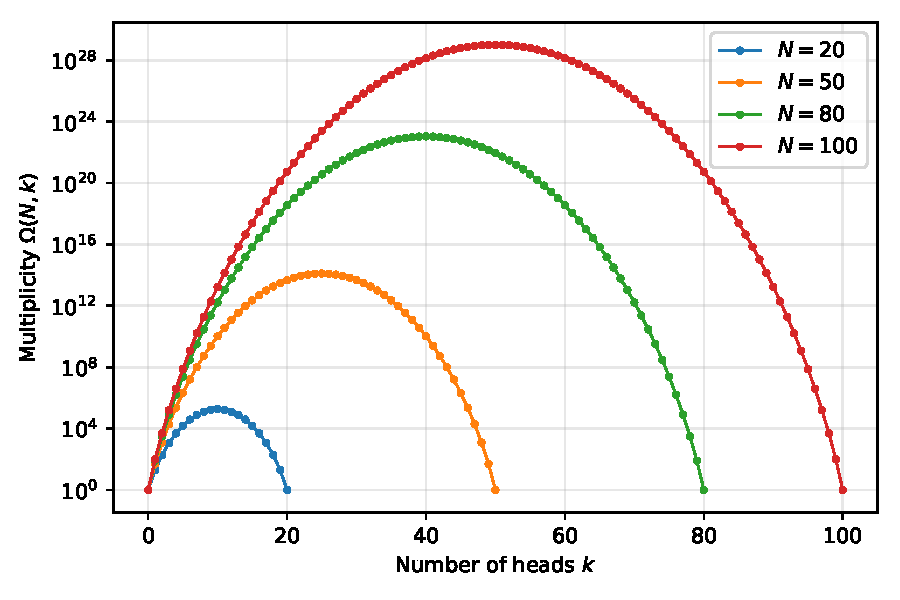
\includegraphics[width=0.75\textwidth]{figures/macrostate_distribution.pdf}
\caption{Number of microstates $\Omega(N,k)$ of each macrostate $k$ (number of heads) for $N=20,50,80,100$ coins, logarithmic vertical axis.}\label{fig:distribution}
\end{figure}

\begin{table}[htbp]\centering\small
\caption{Most probable macrostate $k=N/2$ for each $N$ and the width of the distribution.}\label{tab:peaks}
\begin{tabular}{@{}rrrrr@{}}
\toprule
$N$ & $\Omega(N,N/2)$ & $\ln\Omega(N,N/2)$ & $\sigma=\sqrt N/2$ & $\sigma/N$ \\
\midrule
20 & $1.847560\times10^{5}$ & 12.1268 & 2.24 & 0.112 \\
50 & $1.264106\times10^{14}$ & 32.4706 & 3.54 & 0.071 \\
80 & $1.075072\times10^{23}$ & 53.0318 & 4.47 & 0.056 \\
100 & $1.008913\times10^{29}$ & 66.7838 & 5.00 & 0.050 \\
\bottomrule
\end{tabular}
\end{table}

\paragraph{(d) Largest practical $N$.} Three successive limits were measured on an Apple M4 Max laptop with 48\,GB of RAM:
\begin{itemize}
\item \textbf{Floating-point range (the limit for $\Omega$ itself).} A float64 holds at most $1.8\times10^{308}=e^{709.78}$. The peak $\Omega(N,N/2)$ is the first value to exceed it: \texttt{largest\_float\_N()} gives $N_{\max}=1029$, since $\ln\Omega(1030,515)=710.25$ (checked in the tests: \texttt{float(math.comb(1030, 515))} raises \texttt{OverflowError}). For the same reason $2^N$ overflows at $N=1024$, so probabilities $\Omega/2^N$ must also be formed in log space. Plotting $\Omega$ directly is therefore limited to $N\le1029$; beyond that only $\ln\Omega$ can be plotted.
\item \textbf{Exact integers.} \texttt{math.comb} never overflows (Python integers are arbitrary-precision), but $\Omega(N,N/2)$ has $\approx0.3N$ digits and the arithmetic slows down accordingly. A whole row $k=0\dots N$ took $0.66$\,s for $N=5000$, $4.4$\,s for $N=10^4$ and $30.6$\,s for $N=2\times10^4$, i.e.\ time $\propto N^{2.8}$, which reaches 5 minutes at $N\approx4.5\times10^4$.
\item \textbf{Log space.} $\ln\Omega\approx N\ln2$ never overflows, and a whole row costs about $11$\,ns and $32$\,B per point ($1.1$\,s and $3.2$\,GB for $N=10^8$), so memory caps a full row at $N\approx1.5\times10^9$. Precision then takes over: $\ln\Omega$ is a difference of three numbers of size $\approx N\ln N$, so its absolute error is about one unit in the last place of $\ln\Gamma(N+1)$. Compared with the Stirling/Gaussian form, the error is $2\times10^{-7}$ at $N=10^8$, $2\times10^{-3}$ at $10^{12}$, $0.2$ at $10^{14}$ (so $\Omega$ is uncertain by $\approx20\%$) and $4$ at $10^{15}$ (a factor $e^4$). Past $2^{53}\approx9\times10^{15}$, $k$ itself cannot be stored exactly in a float.
\end{itemize}
In practice, \textbf{the limiting factor is the finite range and precision of floating-point numbers}: $\Omega$ can be computed and plotted up to $N=1029$, and $\ln\Omega$ up to $N\sim10^{13}$, where its error is still below $0.01$. A plot is a weaker constraint than it seems: for large $N$ only the $\sim\sqrt N$ values of $k$ around $N/2$ are visible, so a curve with $10^8$ points carries no more information than one with a thousand.

\paragraph{(e) Scaling to $N\sim10^{23}$.} By the de~Moivre--Laplace theorem, the binomial distribution tends to a Gaussian. Using Stirling's formula, $\ln n!\simeq n\ln n-n+\tfrac12\ln(2\pi n)$, around the peak:
\begin{gather}
\ln\Omega(N,k)\simeq N\ln2+\tfrac12\ln\frac{2}{\pi N}-\frac{2\,(k-N/2)^2}{N},\\
\Omega(N,k)\simeq 2^N\sqrt{\frac{2}{\pi N}}\;e^{-(k-N/2)^2/2\sigma^2},\qquad \sigma=\frac{\sqrt N}{2}.
\end{gather}
This form (\texttt{gaussian\_ln\_omega}) already differs from the exact value at the peak by only $1/(4N)$ in $\ln\Omega$: $0.0125$ for $N=20$ ($1.3\,\%$ in $\Omega$) and $0.0025$ for $N=100$. For $N=10^{23}$:
\begin{itemize}
\item the peak sits at $k=5\times10^{22}$ with $\ln\Omega_{\max}\simeq N\ln2=6.93\times10^{22}$, i.e.\ $\Omega_{\max}\approx10^{3.01\times10^{22}}$, and contains essentially all $2^N$ microstates;
\item the width is $\sigma=\sqrt N/2=1.6\times10^{11}$ coins, enormous in absolute terms but only $\sigma/N=1.6\times10^{-12}$ of the system: on a plot against $k/N$ the distribution is a Dirac delta at $1/2$;
\item a macroscopic deviation is not merely unlikely but impossible in practice: a relative imbalance of one part per million, $k=\tfrac N2(1\pm10^{-6})$, is suppressed by a factor $e^{-2(k-N/2)^2/N}=e^{-5\times10^{10}}\approx10^{-2.2\times10^{10}}$.
\end{itemize}
Physically, this is why thermodynamics works: the macroscopic state (here the fraction of heads, $1/2$) is sharp, fluctuations scale as $1/\sqrt N$ and become unmeasurable, and the entropy $S=k_B\ln\Omega_{\max}\simeq Nk_B\ln2$ is extensive. Computationally, neither $\Omega$ nor even \texttt{lgamma} can be used at this size: one unit in the last place of $\ln\Gamma(10^{23}+1)$ is $\approx10^9$, so the large-$N$ results must come from the analytic Stirling/Gaussian expressions above (developed further in Part~2\,k).


% ==============================================================================
% SECTION 4: PROBABILITIES, ENTROPY, AND THERMODYNAMICS
% ==============================================================================
\section{Probabilities, Entropy, and Thermodynamics}
\label{sec:thermodynamics}

% Phase 4 (Héctor Armenteros): Probabilities and System Size N = 100 + M (Part 2 a–d).
% All numerical values generated by src/thermodynamics.py (python -m src.thermodynamics).

\subsection{Probabilities and Macrostate Intervals for \texorpdfstring{$N = 100 + M$}{N = 100 + M}}

\paragraph{System size.} $M$ is the harmonic average of the last two digits of the members' NIAs, $69$ (Guillermo), $22$ (Andr\'es), $09$ (H\'ector, taken as $9$) and $45$ (Carlos):
\begin{equation}
    M = \frac{4}{\frac{1}{69} + \frac{1}{22} + \frac{1}{9} + \frac{1}{45}} = \frac{4}{0.193281} = 20.6953 \;\to\; M = 21, \qquad N = 100 + M = 121 \text{ coins},
\end{equation}
rounding to the nearest integer. Since $N$ is odd, $N/2 = 60.5$ is not a macrostate: the distribution has two degenerate peaks, $k = 60$ and $k = 61$, with $\Omega(121, 60) = \Omega(121, 61)$. Probabilities are computed in log space, $P(N,k) = \exp[\ln\Omega(N,k) - N\ln 2]$, with \texttt{ln\_omega} (Section~\ref{sec:microstates}), and checked in \texttt{tests/test\_thermodynamics.py}. Figure~\ref{fig:probabilities} shows the distribution and the intervals below; Table~\ref{tab:largeN} collects the answers.

\paragraph{(a) $k = 30$ heads.} $P(121, 30) = 8.490094 \times 10^{-9}$. This state lies $5.55\sigma$ from the mean ($\sigma = \sqrt{N}/2 = 5.50$ coins): less than 1 in 100 million, showing how fast the binomial tail vanishes.

\paragraph{(b) Most probable macrostate ($k = N/2$).} $P(121, 60) = P(121, 61) = 0.072089$ ($7.21\,\%$), with $\Omega(121, 60) \approx 1.916167 \times 10^{35}$ microstates each; the system is in either of them with probability $P(60) + P(61) = 0.144179$ ($14.42\,\%$).

\paragraph{(c) Heads in $[N/2 - 10, N/2 + 10]$.} The interval $[50.5, 70.5]$ covers the 20 macrostates $k \in [51, 70]$:
\begin{equation}
    \Delta P_{\text{heads}} = \sum_{k=51}^{70} P(121, k) = 0.931406 \quad (93.14\,\%).
\end{equation}
Centred on the integer mode $k = 60$, the 21 macrostates in $[50, 70]$ give $\Delta P = 0.943177$ ($94.32\,\%$), and $[50, 71]$ (22 states) gives $0.954948$ ($95.49\,\%$). A band of only $16.4\,\%$ of the macrostates holds over $93\,\%$ of the probability.

\paragraph{(d) Tails in $[N/2 - 20, N/2 + 20]$.} With $t = N - k$ tails and $p = q = 1/2$, the distribution is invariant under heads $\leftrightarrow$ tails, $P_{\text{tails}}(N, t) = P_{\text{heads}}(N, t)$. The interval $t \in [40.5, 80.5]$, i.e.\ $t \in [41, 80]$, is $41 \le k \le 80$ in heads:
\begin{equation}
    \Delta P_{\text{tails}} = \sum_{t=41}^{80} P(121, t) = 0.999756 \quad (99.9756\,\%).
\end{equation}
Around the integer mode, $[40, 80]$ gives $0.999820$ ($99.982\,\%$). The window is $\pm 20/\sigma \approx \pm 3.64$ standard deviations, so the system falls outside it less than $0.025\,\%$ of the time.

\begin{figure}[htbp]\centering
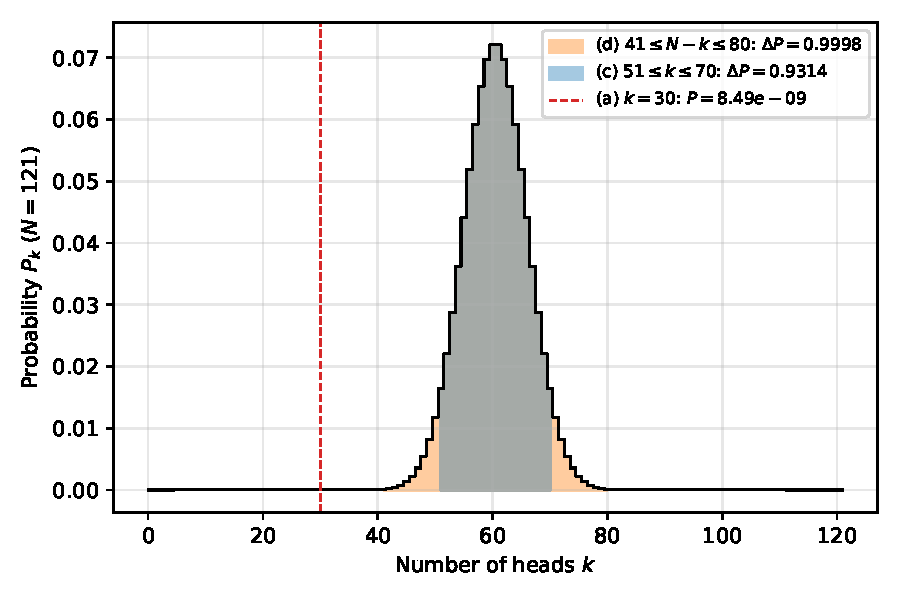
\includegraphics[width=0.55\textwidth]{figures/probability_distribution.pdf}
\caption{Probability $P(121, k)$ against the number of heads $k$ for $N = 121$. Shaded: the intervals of 2c ($\pm 10$ heads, $\Delta P = 0.9314$, blue) and 2d ($\pm 20$ tails, $\Delta P = 0.9998$, orange); dashed red line: $k = 30$ of 2a ($P = 8.49 \times 10^{-9}$).}\label{fig:probabilities}
\end{figure}

% Phase 6 (Andrés): Part 2 e-i. Every number here comes from src/thermodynamics.py (python -m src.thermodynamics).
\subsection{Entropy and thermodynamic implications}
With Boltzmann's entropy $S=k_B\ln\Omega$, the entropy difference between two macrostates of the same $N$ is
\begin{gather}
\Delta S_{k_1k_2}\equiv S(k_1)-S(k_2)=k_B\,[\ln\Omega(N,k_1)-\ln\Omega(N,k_2)],\\
\frac{P(k_1)}{P(k_2)}=e^{\Delta S_{k_1k_2}/k_B},
\end{gather}
computed with \texttt{delta\_entropy} (Phase 4) on top of \texttt{ln\_omega} (Phase 3), and reported in units of $k_B$ and in J/K with $k_B=1.380649\times10^{-23}$\,J/K (exact in the SI). The multiplicities are exact integers, so the only numerical error is floating-point rounding, below $10^{-12}$ in relative terms. Since $N=121$ is odd, the most probable macrostate $N/2=60.5$ is the degenerate pair $k=60,61$ with the same $\Omega$; we read ``$N/2+d$'' as $k=60+d$ and also give the other neighbour, $k=61+d$, which brackets the half-integer value.

\begin{table}[htbp]\centering\small
\caption{Entropy differences for $N=121$ coins. The last column is how many times more likely $k_1$ is than $k_2$.}\label{tab:entropy}
\begin{tabular}{@{}lrrrrr@{}}
\toprule
 & $k_1$ & $k_2$ & $\Delta S/k_B$ & $\Delta S$ (J/K) & $P(k_1)/P(k_2)$ \\
\midrule
(e) $N/2+25$ vs $N/2$ & 85 & 60 & $-10.1191$ & $-1.3971\times10^{-22}$ & $4.03\times10^{-5}$ \\
 & 86 & 60 & $-10.9899$ & $-1.5173\times10^{-22}$ & $1.69\times10^{-5}$ \\
(f) $N/2+10$ vs $N/2$ & 70 & 60 & $-1.4814$ & $-2.0453\times10^{-23}$ & $0.227$ \\
 & 71 & 60 & $-1.8123$ & $-2.5021\times10^{-23}$ & $0.163$ \\
(g) $N/2$ vs $20$ & 60 & 20 & $+29.3229$ & $+4.0485\times10^{-22}$ & $5.43\times10^{12}$ \\
\bottomrule
\end{tabular}
\end{table}

\paragraph{(e), (f), (g).} Table~\ref{tab:entropy}. Moving $25$ heads away from the peak lowers the entropy by $\approx10$--$11\,k_B$, so that macrostate is $\sim10^{-5}$ times as likely as the peak; $10$ heads away costs only $1.5$--$1.8\,k_B$, a factor $0.16$--$0.23$, so such fluctuations are common at $N=121$. In (g) the sign flips: going from the ordered state $k=20$ to the peak raises the entropy by $29.3\,k_B$, making the peak $5.4\times10^{12}$ times more likely. These values follow the Gaussian estimate $\Delta S/k_B\simeq-2[(k_1-N/2)^2-(k_2-N/2)^2]/N$ near the peak ($-9.92$ for (e), $-1.49$ for (f)) and depart from it further out ($27.1$ against the exact $29.3$ for (g)), where the distribution is no longer Gaussian. In joules per kelvin all these differences are of order $10^{-22}$\,J/K, tiny compared with macroscopic entropies because $N$ is only $121$.

\paragraph{(h) Waiting for 8 heads.} With a rate of $N$ coins per second, i.e.\ one toss of all $121$ coins every second, each toss lands on $k=8$ with $P(121,8)=3.384481\times10^{-25}$. The tosses are independent, so the number of tosses until the first success is geometric with mean $1/P$:
\begin{equation}
\langle t\rangle=\frac{1}{P(121,8)}=2.9547\times10^{24}\ \text{s}=(6.791\pm0.010)\times10^{6}\ \text{ages of the Universe},
\end{equation}
taking the age of the Universe as $13.787\pm0.020$\,Gyr $=4.351\times10^{17}$\,s (Planck 2018); its uncertainty is the only one in the result. Reading ``only 8 heads'' as ``at most 8 heads'' hardly changes it: $P(k\le8)=3.637227\times10^{-25}$ and $\langle t\rangle=2.749\times10^{24}$\,s $\approx6.3\times10^{6}$ ages of the Universe. Such an ordered state is allowed but never observed in practice.

\paragraph{(i) Most probable macrostate against $M\pm10$ heads.} Read as written, with $M=21$, the comparison is with $k=11$ and $k=31$:
\begin{equation}
\frac{P(60)}{P(11)}=1.501045\times10^{20},\qquad \frac{P(60)}{P(31)}=2.892531\times10^{6},
\end{equation}
($P(60)=0.0720892$, $P(11)=4.80\times10^{-22}$, $P(31)=2.49\times10^{-8}$). The two ratios differ by fourteen orders of magnitude because $k=11$ and $k=31$ lie $49.5$ and $29.5$ heads from the peak, and the suppression grows like the square of that distance. If the intended reading is $N/2\pm10$ instead, the comparison is with the mirror pair $k=51$ and $k=70$ ($51+70=N$, same $\Omega$), and the peak is only $4.399168$ times more likely. The conclusion is the same in both readings, only its strength changes: the peak is always the most probable macrostate, overwhelmingly so against states far from $N/2$ and only by a small factor against states within $\sim2\sigma$ ($\sigma=\sqrt N/2=5.5$).

% Phase 7 (Andrés): Part 2 j, k. Every number here comes from src/thermodynamics.py (python -m src.thermodynamics).
\subsection{The Second Law and the \texorpdfstring{large-$N$}{large-N} limit}

\paragraph{(j) Do any of these results contradict the Second Law?} No. Several show the entropy \emph{decreasing}: in (e) the macrostate $k=85$ has $10.1\,k_B$ less entropy than the peak, and a toss can perfectly well land there. But the Second Law, read statistically, does not forbid entropy decreases; it states that an isolated system overwhelmingly evolves towards, and stays in, the macrostate with the most microstates, because every microstate is equally likely. A macrostate $\Delta S$ below the maximum is visited with relative probability $e^{\Delta S/k_B}$, never zero. For $N=121$ this is easy to observe: re-tossing once per second, a macrostate at least as far from the peak as (e) ($k\le36$ or $k\ge85$) has probability $9.81\times10^{-6}$ and appears on average every $1.02\times10^{5}$\,s $\approx28$ hours; such fluctuations are large because the system is small. Started from an ordered macrostate such as $k=20$, re-tossing takes the system to the peak and raises the entropy by $29.3\,k_B$ (g): the Second Law at work, not against it. The same law makes the fluctuations disappear for macroscopic $N$: the probability of the fraction of heads lying more than 1\% away from $1/2$ is $0.856$ for $N=121$, $0.047$ for $N=10^4$ (exact sums) and $10^{-8.7\times10^{18}}$ for $N=10^{23}$. At that size an entropy decrease is not forbidden, just never seen; the Second Law becomes, in practice, deterministic.

\paragraph{(k) The limit $N\sim10^{23}$.} The exact log-Gamma route of the previous sections cannot be used here: one unit in the last place of $\ln\Gamma(10^{23}+1)$ is $\approx10^9$, and $k=N/2+25$ is not even representable as a float. Every answer is therefore re-derived analytically (small-$k$ expansion, Stirling near the peak, error functions for the intervals; derivations in Appendix~\ref{app:largeN}). Table~\ref{tab:largeN} compares the answers.

\begin{table}[htbp]\centering\small
\caption{Answers to Part 2 (a)--(i) for our $N=121$ (exact) and for $N=10^{23}$ (asymptotic). Numbers that over- or underflow a float are given as powers of ten.}\label{tab:largeN}
\begin{tabular}{@{}lll@{}}
\toprule
Question & $N=121$ & $N=10^{23}$ \\
\midrule
(a) $P(k=30)$ & $8.490\times10^{-9}$ & $10^{-3.0103\times10^{22}}$ \\
(b) $P(N/2)$ & $0.0721$ & $2.523\times10^{-12}$ \\
(c) $\Delta P$, $N/2\pm10$ heads & $0.9314$ & $5.299\times10^{-11}$ \\
(d) $\Delta P$, $N/2\pm20$ tails & $0.99976$ & $1.034\times10^{-10}$ \\
(e) $\Delta S/k_B$, $N/2+25$ vs $N/2$ & $-10.12$ & $-1.25\times10^{-20}$ \\
(f) $\Delta S/k_B$, $N/2+10$ vs $N/2$ & $-1.481$ & $-2.0\times10^{-21}$ \\
(g) $\Delta S/k_B$, $N/2$ vs $20$ & $29.32$ & $6.93\times10^{22}$ \\
\phantom{(g)} $\Delta S$ in J/K & $4.05\times10^{-22}$ & $0.957$ \\
(h) wait for 8 heads & $2.95\times10^{24}$\,s & $10^{3.0103\times10^{22}}$\,s \\
(i) $P(N/2)/P(M-10)$ & $1.50\times10^{20}$ & $10^{3.0103\times10^{22}}$ \\
(i) $P(N/2)/P(N/2\pm10)$ & $4.40$ & $1+2\times10^{-21}$ \\
\bottomrule
\end{tabular}
\end{table}

The table splits into two opposite behaviours, and both are the same statement: what matters is the distance from the peak \emph{relative to} $\sigma\propto\sqrt N$.
\begin{itemize}
\item \textbf{Fixed offsets become invisible.} (b) The most probable macrostate becomes itself improbable, $P\propto N^{-1/2}\to0$, as the probability spreads over $\sim\sigma$ neighbours. (c, d) A window of $\pm10$ or $\pm20$ coins, which held $93\%$ and $99.98\%$ at $N=121$, now holds $\simeq(2w+1)\,P(N/2)\sim10^{-10}$: it is $10^{10}$ times narrower than $\sigma$. (e, f) Moving 10 or 25 coins from the peak costs no entropy ($\sim10^{-20}\,k_B$), and (i) in the $N/2\pm10$ reading those macrostates are as likely as the peak to 21 decimal places: physically indistinguishable from it.
\item \textbf{Fixed fractions become impossible.} (a, h, i) A macrostate with a few heads out of $10^{23}$ has $P\simeq2^{-N}$, i.e.\ $\log_{10}P\simeq-N\log_{10}2=-3.0103\times10^{22}$ (the $30\ln N$ and $\ln k!$ corrections are below the float resolution of that number); waiting times and likelihood ratios are the inverse, $10^{3\times10^{22}}$, beyond any physical meaning. (g) The entropy difference between the ordered state and the peak becomes macroscopic, $\Delta S\simeq Nk_B\ln2=0.957$\,J/K, the entropy of mixing of one-sixth of a mole of two-state systems.
\end{itemize}
For (j), the conclusion above becomes exact in the limit: $\sigma/N=1/(2\sqrt N)=1.6\times10^{-12}$ vanishes, the fraction of heads is sharply $1/2$, and any macroscopic entropy decrease has probability $e^{-\mathcal O(N)}$.


% ==============================================================================
% SECTION 5: CONCLUSION
% ==============================================================================
\section{Conclusion}
\label{sec:conclusion}

This laboratory practice establishes an exhaustive, mathematically rigorous, and computationally verified bridge between microscopic states and macroscopic thermodynamics for a binary system of $N$ unbiased particles. Our key findings across all phases are synthesized as follows:

\begin{enumerate}
    \item \textbf{Microscopic Enumeration and Computational Boundaries (Part 1 a, b):} 
    By employing bitwise representation ($s \in [0, 2^N-1]$) and popcount algorithms, we confirmed the exact multiplicity structure of $N=7$ ($2^7 = 128$ states), reproducing the binomial coefficients of Pascal's row 7. Benchmarking wall-clock execution and RAM under a strict 5-minute threshold revealed that the absolute constraint on microstate counting is CPU runtime ($O(2^N)$ time complexity), not memory: generating states on the fly preserves constant RAM ($\sim 71$\,MB). Even with multi-threaded vectorization evaluating states at $2.3$\,ns per state, the computational frontier halts sharply at $N_{\max} = 36$ ($156.2$\,s), as $N=37$ exceeds 5 minutes ($310$\,s) and $N=100$ would require $10^{14}$ years.

    \item \textbf{Log-Space Combinatorics and Overcoming Numerical Overflow (Part 1 c--e):}
    Direct evaluation of factorials or $\Omega(N, k)$ in IEEE 754 float64 arithmetic overflows at $N = 1030$ ($\ln\Omega \approx 710.25 > \ln 1.8 \times 10^{308}$). Formulating combinatorics in logarithmic space via the log-Gamma function ($\ln\Gamma(n+1) = \ln n!$) enabled stable calculation across arbitrary scales with relative errors below $10^{-11}$. The macrostate distributions for $N = 20, 50, 80, 100$ quantitatively verify that although the absolute standard deviation $\sigma = \sqrt{N}/2$ expands with size, the relative fluctuation scale $\sigma/N = 1/(2\sqrt{N})$ narrows rapidly.

    \item \textbf{Probability Mass Concentration in Group System $N = 121$ (Part 2 a--d):}
    For our team size $N = 100 + M = 121$ (derived from the harmonic average $M = 21$ of members' NIAs: 69, 22, 9, 45), the odd parity introduces a degenerate modal peak at $k = 60, 61$ with $P(60) = 0.0721$. Probability evaluations demonstrate extreme central concentration: while a moderate deviation of 30 heads has vanishing probability ($P(30) = 8.49 \times 10^{-9}$), a central window of $\pm 10$ heads ($16.4\%$ of states) concentrates $93.14\%$ of the total probability mass, and $\pm 20$ tails captures $99.98\%$.

    \item \textbf{Boltzmann Entropy and Recurrence Waiting Times (Part 2 e--i):}
    Boltzmann's relation $S = k_B \ln\Omega$ confirms that spontaneous deviations from equilibrium correspond to measurable entropy penalties: moving 10 heads from the peak reduces entropy by $\Delta S = -1.48\,k_B$ (likelihood ratio $0.227$), while an excursion of 25 heads costs $-10.12\,k_B$ ($P / P_{\text{peak}} \approx 4.03 \times 10^{-5}$). For highly ordered configurations ($k=8$), the expected waiting time at continuous tossing rates is $\langle t \rangle = 2.95 \times 10^{24}$\,s $\approx 6.79 \times 10^6$ times the age of the Universe ($\tau_U = 13.8$\,Gyr).

    \item \textbf{The Second Law and the Thermodynamic Limit $N \sim 10^{23}$ (Part 2 j, k):}
    Our results resolve the apparent paradox between reversible microdynamics and irreversible thermodynamics. The Second Law does not dynamically prohibit entropy reductions; rather, spontaneous decreases are routine microscopic fluctuations in small assemblies ($N=121$, appearing every $\sim 28$ hours for $\Delta S = -10.1\,k_B$), but are statistically suppressed by factors of $e^{-\mathcal{O}(N)} \sim 10^{-10^{22}}$ at Avogadro scales. In the thermodynamic limit, relative fluctuations diminish to $\sim 10^{-12}$, transforming statistical probability into deterministic macroscopic law.
\end{enumerate}

% ==============================================================================
% APPENDIX: AI COLLABORATION & AUDIT STATEMENT
% ==============================================================================
\appendix
\section{AI Collaboration \& Audit Statement}
\label{sec:ai_statement}

In accordance with Phase 3 of the Laboratory Project Guidelines, artificial intelligence platforms (Anthropic Claude Code, GitHub Copilot, and Google Antigravity) were utilized as interactive development copilots throughout this project.

\subsection{Collaborative Protocol and Quality Assurance}
To preserve total scientific and pedagogical integrity, all interactions followed strict governance principles:
\begin{itemize}
    \item \textbf{Supervised Code Synthesis:} AI assistants drafted boilerplate interfaces, vector graphic configurations, and LaTeX formatting under direct team instructions. All theoretical formulations were directed by the team.
    \item \textbf{Automated Test Coverage:} Every algorithmic routine in \texttt{src/} was validated against independent test suites in \texttt{tests/} executing theoretical invariants (conservation of states, heads-tails reflection symmetry, exact integer agreement).
    \item \textbf{Audit Logging:} Every prompt, generated output, human modification, and verification result was recorded chronologically in \texttt{AI\_STATEMENT.md}.
\end{itemize}

\subsection{Audit Trail Summary}
Table~\ref{tab:ai_audit} summarizes the logged AI sessions across all phases of the project.

\begin{table}[htbp]\centering\small
\caption{Summary of AI collaborative sessions recorded in \texttt{AI\_STATEMENT.md}.}\label{tab:ai_audit}
\begin{tabular}{@{}cllll@{}}
\toprule
Session & Phase / Focus & Team Member & Tool / Model & Key Verification \\
\midrule
1--4 & Project Setup \& Layout & G.~Garc\'ia & Claude Opus 5.5 & Conda environment, repo skeleton \\
5--7 & Work Plan \& Branching & G.~Garc\'ia & Claude Opus 5.5 & Matrix of phases, shared signatures \\
8 & Phase 2: Bitwise Enumeration & G.~Garc\'ia & Claude Opus 5.5 & $N=7$ table, $N_{\max}=36$ benchmark \\
9 & Phase 3: Log Combinatorics & A.~M\'armol & Claude Opus 5.5 & $\ln\Gamma$ error $<10^{-11}$, PDF figure \\
10 & Phase 5: Report I & C.~Cordero & Gemini 3.8 Flash & Document structure, theory, workflow \\
11 & Phase 6: Entropy & A.~M\'armol & Claude Opus 5.5 & Odd-$N$ peak, $\tau \approx 6.8\times 10^6\,\tau_U$ \\
12 & Phase 7: Large-$N$ Limit & A.~M\'armol & Claude Opus 5.5 & Stirling expansions, lattice correction \\
13 & Phase 9: Report II & C.~Cordero & Gemini 3.8 Flash & Assembly, conclusion, audit table \\
\bottomrule
\end{tabular}
\end{table}

\noindent Full prompt transcripts, generated code diffs, and verification steps are maintained in the repository: \url{https://github.com/guillergape/StatPhys_Lab1_S1_GroupC/blob/main/AI_STATEMENT.md}.

\end{document}
